\documentclass{article}
\usepackage{CJKutf8}
\usepackage{setspace}
\usepackage[fleqn]{amsmath}
\usepackage[pdftex]{graphicx}
\usepackage{amssymb}
\begin{CJK}{UTF8}{gkai}
\title{\textbf{浅析视觉神经传导通路及大脑对物体的识别}}
\author{万清甫
\and
计算机科学技术学院
}
\begin{document}
\maketitle
\begin{spacing}{1.0}
\begin{abstract}
视觉是人类最重要的感觉,人类70\%以上的信息都来自视觉系统。我们每天看到成千上万的物体,这些视觉信息在大脑中是怎样传递的?大脑是如何识别种类繁多的物体的?本文先介绍了视觉神经传导通路,视觉神经传导是神经系统传导的一个重要组成部分,使人具有视知觉能力。视觉信息从眼睛传递到中枢神经系统后,大脑进一步对信息加工从而识别物体。本文的第二部分主要介绍了大脑如何进行识别,并分析了一个具体的案例。
\end{abstract}
\section{简介}
\ \ \ \ \ 本文的各个部分先介绍每部分的核心内容,然后适当加入一些联想和启发。主要安排如下:\par 
	第一部分主要介绍视觉神经通路的有关信息,介绍了视觉信息如何从眼睛进入到中枢神经系统:光线聚焦到视网膜,视网膜的视神经到外侧膝状体,外侧膝状体到初级视皮质,接着着重介绍了视觉神经通路中各级神经元的感受野特性,其中包括神经节细胞和外侧膝状体神经元的感受野以及简单细胞和复杂细胞的感受野,然后简单提及感受野的启迪意义。 \par 
	第二部分主要介绍皮质视觉区,首先介绍了关于皮质视觉区作用的两种观点:等级结构和分而治之,然后重点介绍了受高级皮层神经细胞启发的计算模型。\par 
	前面两个部分主要介绍的是视觉神经传导通路,包括视觉信息处理的初级(视网膜)、中级(外侧膝状体)、高级(皮质视觉区)部分,在此基础上,第三部分介绍了物体识别的有关信息。首先介绍了与物体识别密切相关的腹侧通路的神经元特性,借此强调这部分通路的神经元对物体识别的重要性,接着以外侧枕区联合体为例详细介绍了大脑特定区域在物体识别中的作用。介绍完具体的腹侧通路神经元和大脑特定区域对物体识别的意义后,从局部到整体,在神经水平上总结了物体在大脑中表征的两种方式,总结分析了物体识别的认知模型。最后,运用前述的物体识别理论具体分析了一个案例:手的检测,并适当地加入神经网络对这个问题的可视化输出说明神经网络和神经系统的联系与区别。\par 
	第四部分总结全文,提出了一些感想。
\section{视觉神经通路}
\ \ \ \ 人是极度依赖视觉的高等动物,我们每天接触成千上万的信息很多来自视觉。视觉信息从眼睛进入到中枢神经系统经过了如下流程:
\subsection{光线聚焦到视网膜}
\ \ \ \	视网膜上有无数的感光细胞,这些细胞的输出经过视网膜中间层的加工,通过视神经传入中枢细胞。其中感光细胞有两种,一种是视锥细胞,一种是是视杆细胞,这两种细胞对光的敏感程度各不相同。这种设计的精妙之处在于,不同环境情况下光的强弱不同,物体之间可能会有自遮挡,不同角度的光照射下来在物体上可能产生阴影,我们希望的是我们不会因为这些因素降低识别物体的能力,如果所有细胞一视同仁就很难不被外界细微因素影响。此外,视锥细胞基本只在中央凹附近,且在日间活动较强。相信大多数人的眼睛看到一个物体首先会不自觉地盯着物体的中央部分,光线经过晶状体投射到视网膜的过程可以看做一个简单的透镜成像,靠近物体中央的部位投影到视网膜上相应的也靠近视网膜的中央即中央凹,对日间强光敏感的视锥细胞分布在中央凹附近有助于人聚焦于物体的中央部位。\par 
	随着计算机视觉的发展,科研人员一直致力于让计算机识别物体,最近微软研究院成功在ImageNet上将计算机识别物体的错误率先后降低至4.94\cite{delving}和3.57\% \cite{deep}, 首次低于人眼5.1\%的错误率。然而,计算机处理的终究是已经经过照相机拍摄处理过后的图像,而人的眼睛是把进入的光线通过晶状体成像在视网膜上,照相机的焦距和晶状体这种天然透镜的焦距不同导致计算机和人眼接收到的物体根本就没有可比性。数以亿计各司其职的视杆视锥细胞可以敏锐地感知光线强弱的变化,甚至可以在黑暗的环境下感知物体的形状,然而此时计算机处理的图像质量已经相当低,灰度的变化量级远远不能满足需求。感光细胞在处理光刺激的时候其实隐含了对物体中央部位的先验知识,在中央附近感知到更多信息,而计算机没法精确地模拟从人眼的视角对不同区域有不同的敏感程度。此外,这些感光细胞中的感光色素在光线暴露下分解触发神经元动作电位,转换为内部神经信号。色素分解、电流变化纯粹是物理和化学层面的反应,是非常不稳定的,企图通过理想的数学公式模拟感知器本身就是非常局限的。
\subsection{视神经到外侧膝状体}
\ \ \ \ 视网膜的输出视神经向外侧膝状体继续传递,然后外侧膝状体传入中枢神经系统。人的视野可以分为左视野和右视野,每只眼球视网膜左侧视神经受到右视野物体刺激,而右侧视神经受到左视野物体刺激。颞侧视神经只往同侧传递,而鼻侧视神经只往对侧传递,这样左眼的颞侧和右眼的鼻侧视神经(均为右视野)将右视野的所有信息传递到大脑左侧半球的外侧膝状体,而左眼的鼻侧和右眼的颞侧视神经(均为左视野)将左视野的所有信息传递到大脑右侧半球的外侧膝状体。
\subsection{外侧膝状体到初级视皮质}
\ \ \ \ 外侧膝状体充当了视神经到大脑皮层的中转站,最后外侧膝状体的轴突延伸到枕叶的初级视皮质。
\subsection{小结}
\ \ \ \ 总而言之,通过鼻侧神经在枕核处的视交叉,来自左视野的视觉信息到达大脑的右边半球,而右视野的视觉信息到达大脑的左边半球。从光线进入到皮质的信息先后经过了晶状体成像、感光细胞输出、视网膜中间层神经元加工、感光细胞加工、外侧膝状体(LGN)细胞加工,这其中每一个环节神经元都对视觉信息进行了加工,每一步都是精妙设计必不可缺的。其中值得注意的是,视网膜输入感光细胞一共有2亿6千万,而输出神经节细胞仅有200万,输入和输出细胞数量的巨大差别体现了视网膜细胞对信息的高度压缩能力。视网膜细胞将高维的数据压缩降低维度,提取出最核心的那些有助于在大脑中建立外部视觉场景的影像信息,而将不那么重要的神经元激活值抑制不再保留,这种思想值得借鉴。
\subsection{视觉神经通路中各级神经元的感受野特性}
\ \ \ \ 如果视网膜上所有空间区域的光刺激都影响到视觉通路中各级神经元的电位变化,这样复杂的连接可能存在相当多的冗余信息,真实的设计是:视觉通路中各级神经元的电位变化等活动受视网膜上某个特定空间区域的光刺激,这个特定的区域称为该细胞的感受野。(receptive field)。感受野一般为同心圆分布,针对感受野到底是什么形状,20世纪80年代以来,很多神经生理学家研究发现部分神经节细胞感受野不是严格意义上的圆形,而是拉长的椭圆形甚至不规则形状(Shou和Leventhal 1989)\cite{hsh}  。\par  以外侧膝状体(或神经节细胞)神经元的感受野为例,感受野以同心圆方式分布,落在感受野内部的光刺激激活细胞发放动作电位,落在外部的光刺激抑制细胞电位变化,而当光线同时位于中心和外周时激活和抑制相互抵消,导致细胞不被激活。可以想见当一束有边界的光线从外周不断移到感受野内部,细胞从被抑制到被激活,势必存在一个边界值,当光线正好经过这条边界时,细胞恰好完成从被抑制到被激活的状态转变。由此可见,和外侧膝状体、神经节细胞这种感受野为同心圆类似的细胞对边缘的变化最感兴趣,当我们看一个物体并试图去识别它时,我们是通过物体边缘的变化、前景和背景分界线的差别等将这个物体与其它物体区别开。\par 
	前面介绍了神经节细胞和外侧膝状体神经元的感受野,那么初级视觉皮层内神经元的感受野是什么样的呢?如将感受野中心位置稍有不同的三个外侧膝状体细胞输出联系到同一个皮质神经元,会发现这个皮质神经元的结构是中央-周围的,Hubel和Wiesel将这种细胞称为简单细胞,初级视皮质的简单细胞的感受野是狭长形的。这种狭长形的结构和前面所述同心圆结构一样,也能敏锐地察觉到边缘的变化。然而不像同心圆结构,如果小光点在同心圆感受野内部,不论其如何旋转,细胞总是激活的,这是由它的圆形结构决定的,然而在初级视皮质简单细胞中,当光刺激以一定角度旋转时会同时跨越兴奋和抑制区域,最终会导致细胞不激活。简单细胞对光的苛刻要求说明它只能接受神经元偏爱的最优方向的光刺激,凡是不是这个最优方向的光刺激它不会做出反应,从而不能很好地提取边缘。人工卷积神经网络(Convolutional Neural Network,CNN)中所谓的神经元,其实类似这种简单细胞,卷积操作每次只对一个小的邻域(小区域)内的像素值有响应,这个邻域是人工神经网络中的”感受野“,它的形状就是简单的狭长形,所不同的是,这里没有光刺激,没有所谓的最优朝向。初级视皮质块中,感受野中心相似,但细胞的最优朝向不断变化,一系列这样的皮质块具有不同的最优朝向,从而可以表示整个空间的光刺激,便于视觉系统全方位地提取边缘信息。相比之下,CNN的神经元只是借用了生物中神经元的概念,而且还是最精简化的神经元。CNN处理的是静态图像,试图优化一个函数,朝着梯度的最优方向下降,而初级视皮质块中遍布的多个最优朝向,简单细胞会被最优朝向的边缘兴奋或抑制,这么多最优朝向总有一个适合于当前的光刺激,当光刺激方位与某个最优朝向相同即匹配时,神经元有强动作电位发放,而不匹配时则不被激活,细胞激活与否是匹配得出的而不是简单暴力计算得出的。\par 
	在初级视觉皮层中还有另外一类细胞被称为复杂细胞,它对其它特征如拐角或边缘终端更敏感,它也有强的方位选择性,只是对刺激具体在哪个位置发生并没有太严格的限制。一个复杂细胞接受若干简单细胞的输入,这些简单细胞的感受野在视网膜上排成一行,无论光刺激发生在哪个简单细胞上,只要在整个复杂细胞的感受野范围内移动,复杂细胞的动作电位都会增加发放频率,也就是说条形的刺激可以在一个小的区域内移动。由上可知,复杂细胞相比简单细胞而言,感受野更大。根据Hubel和Wiesel关于猫的初级视皮层(V1)区的研究,V1区由简单细胞和复杂细胞组成,简单细胞主要响应感受野内的特定边缘刺激,每个复杂细胞以一些简单细胞为输入,以更大的感受野响应特定的边缘刺激,而忽略刺激的精确位置\cite{hsh}。不妨假设有多个复杂细胞,每个复杂细胞的感受野在空间中一个区域逐渐移动并占据这个区域,这样复杂细胞对局部的位置变化具有局部平移不变性,即只要物体在复杂细胞感受野内,无论它在这个区域内怎样平移,复杂细胞总是能被激活。这种位置无关性质的好处在于我们不用关心物体具体分布在视野的哪一个区域,只要物体在那我们的视觉系统就能观察到它。\par 
	CNN试图通过局部卷积核模拟复杂细胞的局部感受野,从图像中提取初级视觉特征如边缘、端点和拐角等,然后通过降采样将图像缩小,降低分辨率,使得网络对输入的局部变换具有一定的不变性。\cite{fcn}中介绍了一种利用CNN进行精确到像素级别的图像分割(每个像素输出属于事先确定好的若干物体类别的概率),其中的网络利用了浅层特征和深层特征。浅层特征图的大小比较大,一个神经元(像素)对应了原图中较小的一个区域,因而这个神经元具有的感受野也比较小,而深层特征一个神经元对应原图较大的一个区域,感受野相对较大。那么感受野大和小的区别究竟在哪里?如前文所述,简单细胞感受野较小,对刺激的空间位置要求严苛;复杂细胞感受野较大,允许刺激在一定范围内移动。由此可知,感受野小的神经元反映的是更加精细的信息,而感受野大的神经元提供了更加粗糙的信息。将低层次细致的信息和高层次模糊的信息合并能更好的反映真实情况,如Figure 1."combine coarse, high layer information with fine, low layer information"\\ \\ \\ \\ \\
\begin{figure}[htbp]
\centering
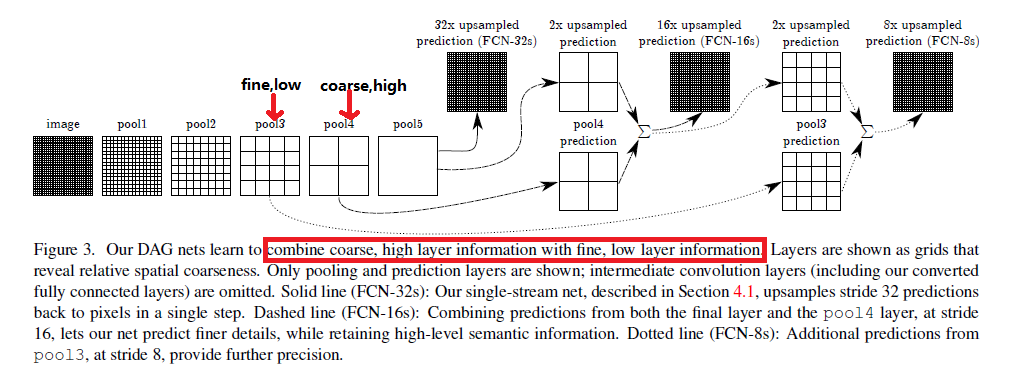
\includegraphics[width=0.70\textwidth]{/home/strawberryfg/brain/fcn.png}
\caption{FCN}
\end{figure}\par 
	随着研究的深入,这种前馈的人工神经网络的层次模型受到了很多质疑和挑战。首先,复杂细胞的输入只有一小部分源自简单细胞,而更多的连接来自同一层次的其它复杂细胞,水平方向、竖直方向的连接构成了复杂的轴突网\cite{jsll}。前馈网络则是前一层和后一层神经元相连,同一层没有连接,为了模型简便易于解决强行将同一层次的生物复杂细胞之间的关联割裂开。同时,在生物神经系统中,还有小部分连接来自形状视觉通路中更高级皮层的细胞。ANN(人工神经网络)中的反馈机制和生物中的千差万别,虽然还没有定论生物反馈连接的具体作用机制对复杂细胞的加工会产生怎样的影响,可以确定的是复杂细胞之间的相互作用对特征加工有很大影响(Plebe),忽略相互作用的ANN显然是不科学的。
\section{皮质视觉区}
\ \ \ \ 前文介绍了视觉信息如何一步一步从眼睛进入外侧膝状体然后到达初级视皮质,人类的大脑包含如此多的皮质视觉区,那么这些视觉区都有什么作用呢?主要有以下两种观点:
\subsection{等级结构}
\ \ \ \ 每一个区域都是对前一个等级的区域提取的特征进行进一步加工,经过处理后生成新的刺激。初级视皮层和纹外皮层的简单细胞负责提取边界,复杂细胞则利用简单细胞的输出提取简单视觉特征(朝向、位置、颜色)以及一些简单的质地、形状、拐角和边缘终端等。然后,高级视皮层如颞下皮层(IT)、颞中回皮层(MT)等加工更加复杂的特征。
\subsection{分而治之}
\ \ \ \ 这种思路采用分治的思想,视觉信息的加工分布给各个视觉区,每一个视觉区只专门处理一种属性。可能某一个区域的神经元对颜色敏感,某一个区域的神经元对亮度敏感,某一个区域的神经元对运动敏感等等。Hubel和Wiesel发现,初级视皮层的某些神经元只对(主要对)输入左眼的视觉刺激起反应,另外一些主要对输入右眼的起反应。继Hubel和Wiesel之后,Livingstone和Hubel\\(1987)对猴的视觉皮层功能结构深入研究,用细胞色素氧化酶染色技术发现,V1区内斑点之间的神经元对特定方位的刺激反应,V2区内暗的窄条纹内神经元对颜色敏感\cite{sjkxyl}……\par 
\subsection{两种观点小结}
\ \ \ \ 第一种观点就像一个链式的环环相扣的生产线,而第二种观点像一个分布式的系统,无论是哪一种观点都说明不同的神经元加工不同的视觉信息,所不同的仅在于分而治之的策略中,形状、颜色、运动、亮度等视觉信息被并行传递,分布给各个独立的神经元,每个神经元加工的信息不依赖于其它神经元,同时并行独立处理,而第一种等级结构存在一个先后顺序,低层级的信息被高层级的神经元加工表征。如今,广泛证据都支持了第二种分而治之的专门化假设。
\subsection{高级皮层神经细胞计算模型}
\ \ \ \ 前文提到很多普通神经网络都不能很好的模拟真实的生物神经系统,Figure 2介绍的Plebe在\cite{attention}提出的V2区神经细胞计算模型,尽管它仍然是层次模型,而不是现在普遍认为的专门化的并行计算模型,并且囿于其解决问题的单一性并没有在工业界普遍应用,但是它的提出还是具有一定的启发意义,主要体现在同一层神经元之间的互相连接。\par 
\begin{figure}[htbp]
\centering
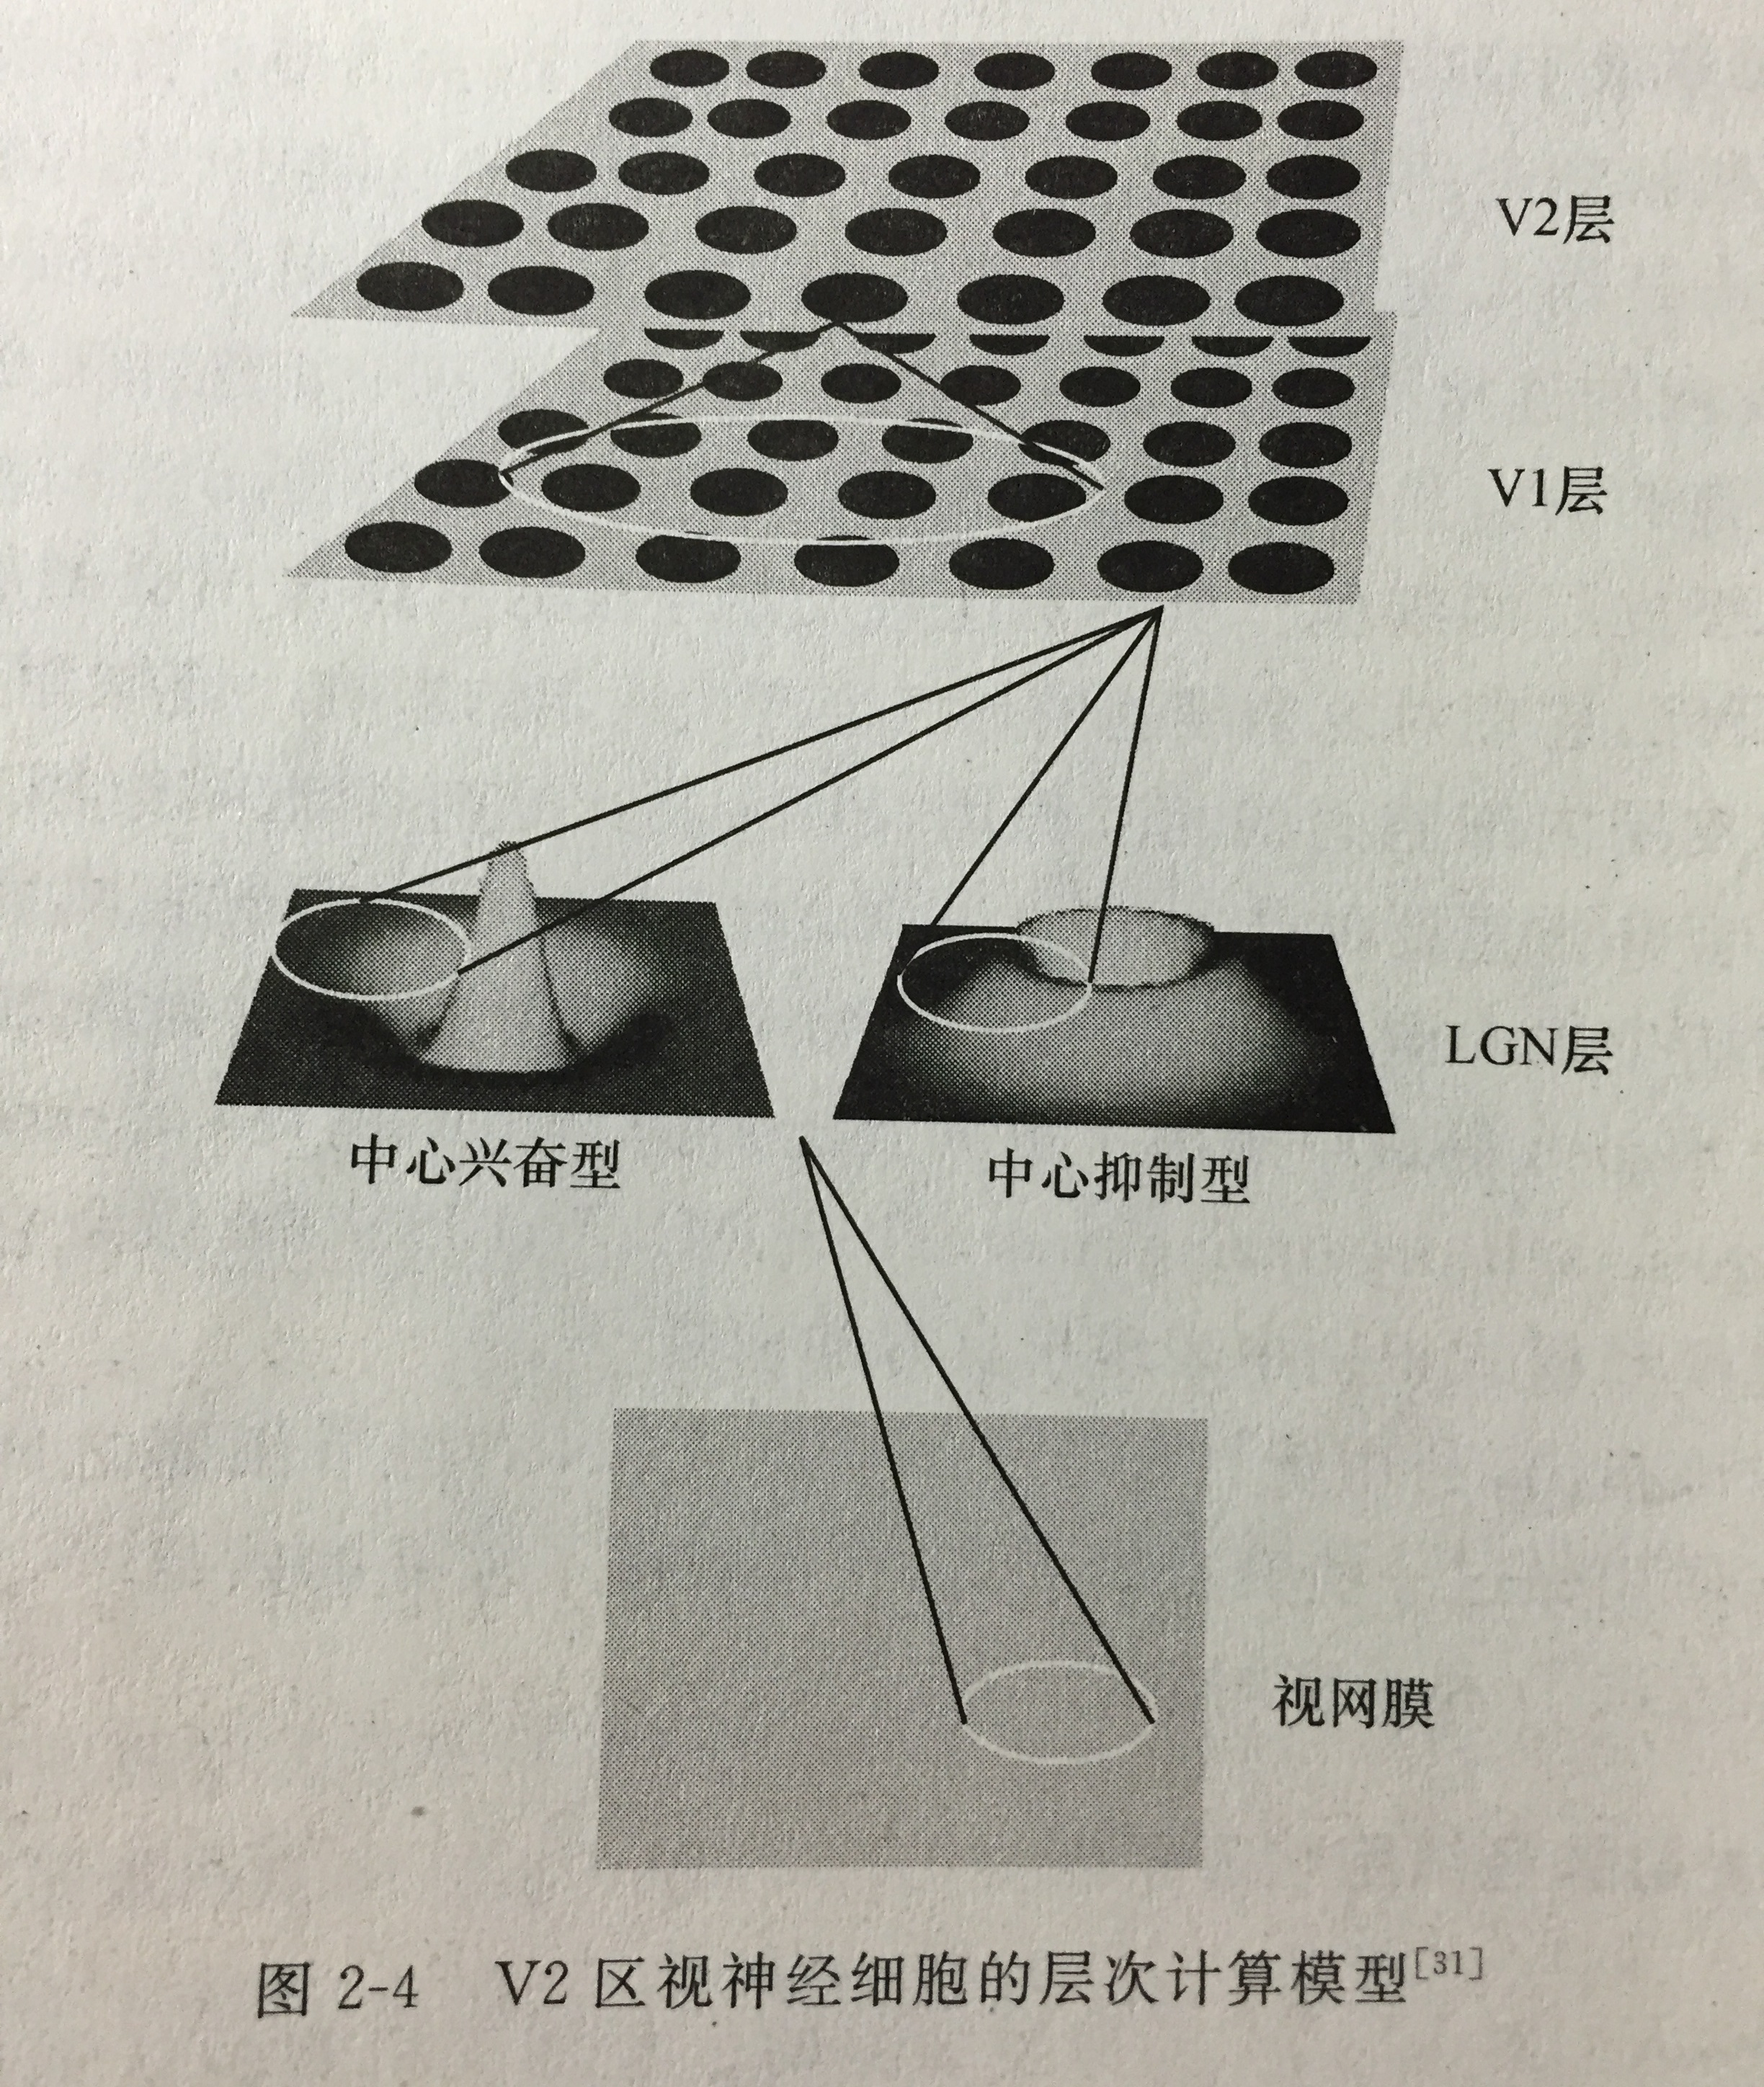
\includegraphics[width=0.4\textwidth]{/home/strawberryfg/brain/V2.JPG}
\caption{V2 计算模型\cite{jsll}}
\end{figure}\par 
LGN层通过中心兴奋(中心-周围感受野结构)和中心抑制滤波器模拟外侧膝状体(LGN)细胞,V1层以LGN输出作为输入,同时在V1层神经元之间还存在同层的侧向互连,这种同一层神经元之间互相连接的网络很罕见,而如前文所述,这正符合复杂细胞在同一层次上相互连接的事实,然后V2层以V1层输出为输入,同时V2层神经元之间也存在同层之间的侧向互连。经过若干次无监督的学习,模拟的V2层神经细胞表现出了对角状刺激的稳定偏好。这个模型只考虑了同一层神经元的相互连接而没有将更高层的神经元连向低层的神经元,主体思想还是把整个问题当成一个naive的数值优化问题,然后利用BP(Back Propagation,反向传播)等方法将高层神经元的兴奋或抑制的影响传递给低层神经元。认知神经科学家提出记忆的连接模型利用到BP算法完成学习,但是在生物神经系统中基本并没有利用这样的反向传播方法。神经元和神经元之间是通过突触连接的,化学物质(神经递质)扩散穿过突出间隙,与突触后模受体分子结合,导致突触后神经元电流产生,神经系统内神经元信号的持续产生构成了一个神经环路\cite{main}。由此可见,生物神经系统中存在神经环路,神经元有电流产生,神经元与神经元之间有化学物质的传送,神经递质的合成、释放等等都涉及复杂的化学变化,所有这些变化都是跟随时间的推移而动态变化的,没有什么恒定遵循的规律,而人工神经网络更倾向于解决一个固定的简化的问题,一旦训练出这个模型,其中的参数就不会变化,对于不同的输入网络不会再自适应地动态改变。
\section{物体识别}
\ \ \ \ 有了视觉神经通路的铺垫后,这一部分开始介绍物体识别。我们身处一个纷繁杂乱的世界,每天面对成千上万的物体,尽管视觉场景非常复杂,我们仍然能在各种严苛的条件下准确地识别出物体。物体识别其实是一个非常复杂的问题,大脑识别物体面临如下诸多问题:\\
1)观看角度的不同导致视网膜上的成像不同,我们从外界观察到的视觉场景非常依赖于我们的观察视角,比如当我们从不同角度观看一辆汽车时,其正面、侧面或后面的成像十分不同。\\
2)即使从一个视角观察一个形状不变的物体,由于照射光源的亮度和角度变化,在物体上形成的阴影也会变化。\\
3)在复杂环境下,物体之间可能会互相遮挡,使得一个物体在视网膜上的成像不完整。\\
4)同一类型的物体之间有很多相似处,容易混淆,需要细粒度的分类。\\
5)不同类别的物体之间有时仅有细微的差异。\par 
尽管存在诸如此类的复杂问题,大脑仍能快速精确地识别物体,这种在各种复杂变换下仍能准确识别物体的能力,又称为\textbf{物体恒常性},对于我们感知和理解这个世界非常重要。\par 
	前文已经介绍了视觉信息从视网膜到皮质的通路以及皮质视觉区的作用,我们不禁想问物体识别在皮质是否存在特定的处理区域?Lesile Ungerleider和Mortimer Mishkin(1982)给出了肯定的答案,他们认为视觉在皮质存在两条通路:腹侧通路(ventral pathway)和背侧通路(dorsal pathway),前者是物体的“什么”通路,决定我们在看的物体是什么东西,后者是物体的“哪里”通路,负责分析物体在空间中分布在什么位置,\textbf{在本文中关注的主要是起主要作用的“什么”通路即腹侧通路。}
\subsection{腹侧通路的神经元特性}
\ \ \ \ 视觉皮层V1和V2神经元严格要求最优朝向,只有满足最优朝向的边界才能被识别出,而较高级的皮质区如V4能识别较复杂的形状。Pasupathy和Connor\\(1999)给猴子不同形状的刺激(不同的角或曲线)并观察V4神经元的反应,结果发现V4对简单细胞处理的那种简单边界或条形刺激反应不明显,而对某一个方向的角有最强反应,具体来说,多数V4神经元对凸起的角有较强反应,对凹陷的角反应不大。此后,Hinkle和Connor(2002)还发现V4不只是在二维平面上对轮廓形状特征敏感,在三维空间中也是如此。\par V4神经元对复杂形状特性的反应说明从对朝向、边界等简单视觉特征敏感的V1到对复杂形状敏感的下颞叶V4等的通路中存在中间加工的过程,负责提取轮廓在不同位置的结构特征,形状特征可能是通过整合不同层级水平(或者不同专门区域)的视觉特征得到的。\cite{lyj} \par 
	众所周知,腹侧通路中更高级的下颞叶皮层在形状加工中起重要的作用,颞叶的神经元具有非常大的感受野。前文提到感光细胞主要在中央凹附近,对视觉信息的中央部位较敏感。这里颞叶的神经元感受野包围中央凹,对中心视觉信息的高度敏感对物体识别是非常重要的,我们通常看一个物体的时候会优先看中央部位,颞叶的神经元在中央凹附近的视觉信息有更大的精确性。而背侧通路的顶叶神经元有60\%不包括中央凹的感受野,对视野的外周等不是中央的位置的刺激更敏感,这也就是为什么顶叶神经元更多的是决定物体在哪里,只需要知道大概而不需要知道物体具体属于哪一种类别。
\subsection{大脑特定区域在物体识别中的作用——以外侧枕区联合体(LOC)为例}
\ \ \ \ 腹侧通路的神经元对提取视觉特征有很大的作用,其实不只是腹侧通路的神经元,脑成像研究表明大脑特定区域在物体识别中也扮演了很重要的角色。举例来说一些脑成像研究表明大脑外侧枕区联合体(LOC)对形状表征起关键作用。Kourtzi和Kanwisher(2001)在\cite{adaption}中采用了神经元适应效应(neural adaption effect)(所谓适应效应就是对于最近没有被观察到的激励的响应比最近被观察到的激励的响应更大)来研究LOC活动究竟与刺激的形状还是和刺激的轮廓有关。轮廓和形状不是一回事,如Figure 3左侧两张图形状相同,但由于竖线的遮挡(occlusion),两个刺激的知觉深度(stereoscopic depth cues)不同,因此二者的局部轮廓不相同;Figure 3右侧两张图轮廓相同,但是形状不同。
\begin{figure}[htbp]
\centering
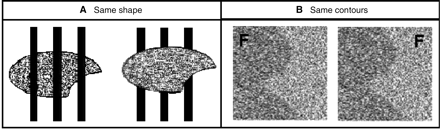
\includegraphics[width=0.4\textwidth]{/home/strawberryfg/brain/shapecontour.png}
\caption{形状和轮廓}
\end{figure}\par 
为了搞清楚LOC表征哪些信息,利用适应效应,\cite{adaption}中的实验一设置了四组子实验,每组子实验的两次刺激顺序呈现,如Figure 4所示。\\ \\ \\ \\ \\ \\ \\ \\ \\
\begin{figure}[htbp]
\centering
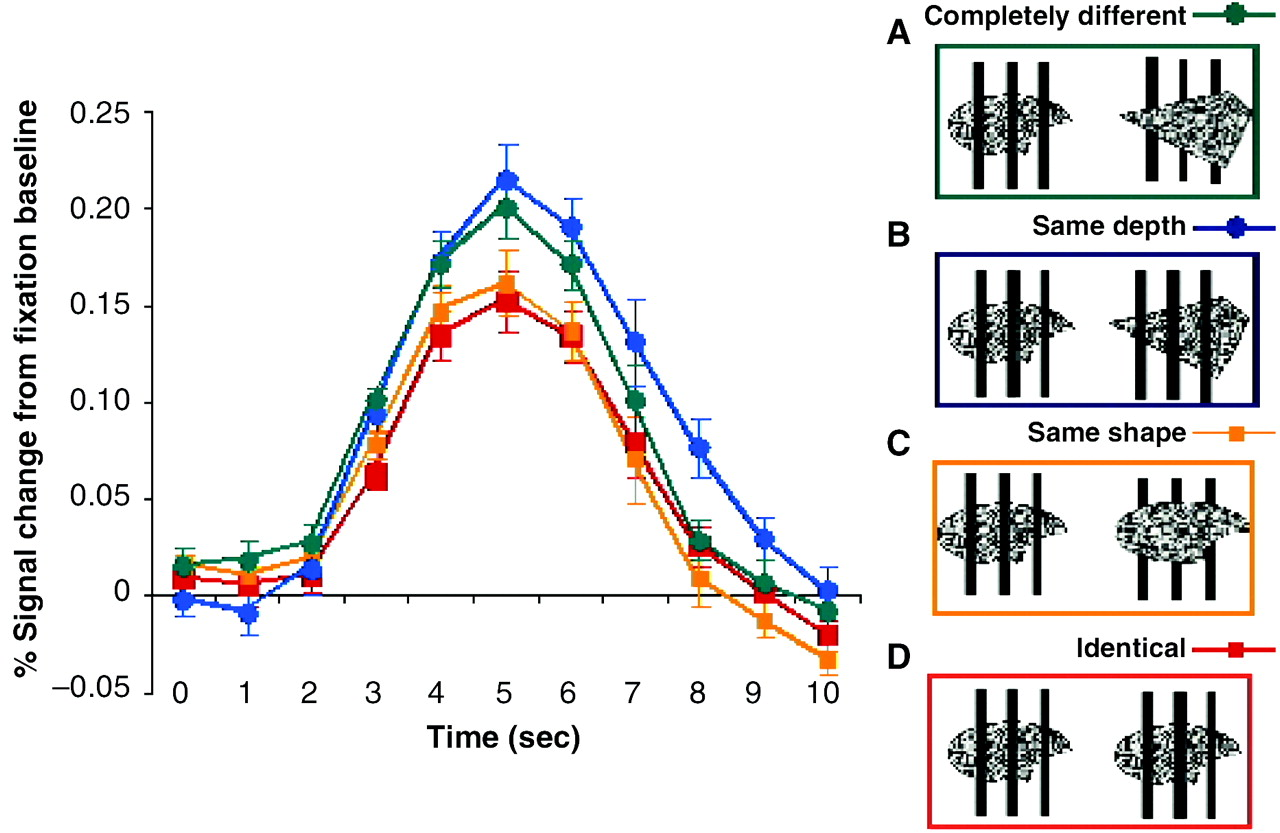
\includegraphics[width=0.6\textwidth]{/home/strawberryfg/brain/LOC.jpg}
\caption{\cite{adaption}中的刺激图形和结果示意图}
\end{figure}\par 
Figure 4的A、B、C、D前后两个刺激知觉深度、轮廓、形状相同/不同的情况如下表:\par 
\begin{tabular}{cccc}  
\hline
编号 & 形状 & 轮廓 & 知觉深度 \\ \hline  
A & 不同 & 不同 & 不同\\ \hline 
B & 不同 & 不同 & 相同\\ \hline 
C & 相同 & 不同 & 不同\\ \hline 
D & 相同 & 相同 & 相同\\ \hline
\end{tabular}
\end{table}\\
(1)对比A和C,在图上可以发现橙黄色的线在绿色的线下方,说明前后激励的形状不同相比前后激励形状相同响应显著下降\par 
(2)对比A和B,紫色的线和绿色的线靠的非常近,说明知觉深度相同与否对在LOC里的响应没有影响,即知觉深度在LOC里没有表征\par 
(3)再对比C和D,橙黄色的线和红色的线非常接近,C和D形状相同,轮廓不同,知觉深度不同,由(2)已知知觉深度不被包含在LOC里面,唯一的解释就是LOC也不表征轮廓信息。\par 
 综上可得出LOC加工的仅仅是抽象的形状信息,而不是低级的轮廓信息。上述的LOC在物体识别中加工形状的例子可以看做是上一节皮质视觉区分而治之专门化处理的一个后续表达。那么,在神经水平上,物体在大脑中是如何表征的呢?
\subsection{神经水平上物体在大脑中表征的两种方式}
\subsubsection{层级编码假说}
\ \ \ \ 类似上一章的等级结构,最底层检测边缘,与简单细胞一样,然后初级的特征被不断编码整合输入更高阶的复杂探测器如拐角、交叉探测器,一层一层加工编码变成更复杂的组合,最后形成一个可被识别的物体。这种假说有一个重要的前提是,对一个物体的知觉是被某个单个细胞编码的,有些生理学家研究发现某个细胞可能表现出对手的特殊偏好,换句话说那个特定细胞是专门识别手这种物体的。当然这个假说的漏洞不言自明,如果单个细胞编码出现问题,细胞坏死等,识别某个特定物体的功能也会随之消失,此外,我们经常遇到新的从未见过的物体,如果每一个物体都有专属的\textbf{知识单元}(负责识别复杂物体的神经元),就像一个特定的神经网络只能处理某一类或者某几类物体,这不符合我们能感知理解新兴物体的现实。
\subsubsection{集群假说}
\ \ \ \ 这种假说认为物体识别不是某个神经元完成的,是多个神经元激活共同作用完成的。每个神经元都可以看做一个复杂的特征探测器, 以人为例,有些神经元对面部轮廓有反应,有些对眼镜有反应,有些对皱纹有反应,有些对脸颊颜色有反应,有些对衣服颜色有反应,有些对头发颜色有反应,等等。当然不是说每个神经元只会对某种物体或者某种特性反应,但是对于某种信息,比如人手的信息,倾向于处理这种信息的神经元都会被激活。上一章皮质视觉区作用的第二种假设认为每个视觉区只处理某种特性,只接受那一种刺激,集群假说似乎不这么认为。根据集群理论,当遇到一个视觉上相似的两个物体时,它们可能都激活许多相同的神经元,产生相同的激活输出,一旦那些表征我们熟悉物体的特性的神经元被激活,我们可能会产生类似熟悉物体的知觉,也就是说我们获得了对新的物体的识别能力。集群假说有颞叶神经元的单细胞研究结果支持,研究表明下颞皮质细胞偏好某种刺激,但它们也能被视觉上相似的刺激激活。\cite{main} \par 

\subsection{物体识别认知模型}
\ \ \ \ 上一节所说的是关于表征物体的两种假说,下面要介绍的是物体识别的三个认知模型。\par 
Warington(1985)提出一个物体识别的解剖学模型,该模型认为物体识别分为两个阶段。第一个阶段进行知觉分类,仅仅根据视觉信息输入和大脑内部储存的关于物体的视觉特征进行一个匹配,这个过程不关心物体的具体功能以及物体的名称是什么,它只对眼球获取到的视觉信息进行加工,克服了感觉信息的变异性即前文所说的物体识别面临的诸多问题;第二个阶段是语义分类,我们的大脑不仅储存了物体的各方面视觉特征,长时记忆中还存储了关于不同物体的功能、名称等信息,语义分类就是在初级的知觉信息基础上加上语义知识,将物体与语言联系起来。现如今很多模拟人脑的研究已经不仅仅满足于像大脑一样挖掘物体的视觉特征,还加入了很多语义标签的先验知识,光知道不同物体外观上的差别还不够,现在的任务更倾向于能挖掘物体中隐藏的语义信息,比如这个物体有什么功能,有什么优缺点,给定一个包含物体的场景图片输入,如何输出一句描述这个物体各种特性的句子,看到若干个物体能否自动用语言描述这些物体共有的特征。Warring的模型仅仅是简单地刻画了我们如何识别物体,可能还需要进一步细化,但这种将知觉和语义联系起来的思想影响了后人。\par 
	融合语义信息的模型还有Farah和McClelland于1991年提出的基于特征的语义系统的联结主义模型结构,用以模拟人们把物体视觉特性和物体特征联系。简单说,输入是外周输入系统,有两个分别是视觉系统和言语系统,每个系统都有若干节点。模型中还存在第二类系统:语义系统,语义系统节点中又包含两种:视觉的和功能的,一类语义知识是基于视觉特征的,如Warington所说的知觉分类阶段获取的语义,另一类语义知识是关于物体的功能的。言语系统节点和语义系统节点互连,视觉系统节点和语义系统节点互连,而言语和视觉节点之间不连接,节点与节点之间的连接权重决定最后整个系统的激活值。不难发现,这个联结主义网络模型其实是在Warington所提出的解剖学模型的基础上改进的一种具体形式化表达,是一种计算理论。\par 
	此外,Farah关于物体识别还提出了一个双加工模型,他认为识别一个目标基于两种形式的分析过程:对整体的分析和对部分的分析。整体加工关注的是整体形状轮廓等,而分析加工强调物体具体的各组成部分,研究表明整体加工对物体识别贡献特别大。
\subsection{案例分析:手的检测与识别}
\ \ \ \ 本文接下来的部分将以一个具体的实际问题来讨论大脑如何检测物体和识别物体:手的检测与识别。手的检测与识别这个问题可以概括为从真实场景中检测出手并还原出手的三维模型。它其实分为检测和识别两个步骤,检测是识别的基础,检测出手后才可以进一步进行手势的识别。大脑是如何检测手的?上一节的层级编码假说中提到有些生理学家发现某个细胞可能表现出对手的特殊偏好,\cite{main}中提到,对下颞皮质的一个细胞进行记录,发现这个细胞对人手的反应最强,而且不论手是什么角度它都能有很强的反应,而当一个盖住手指的手套刺激它时,该细胞仅有微弱的反应,对于其它和手有些类似的比如梳子之类的物体该细胞反应微弱,当手的大小变小时,该细胞的反应和大手的时候相比相对减小。这个实验表明下颞皮质中存在神经元能检测出不同视角的手,且它能把手和与手相似但形状略有不同的物体区别开。\par 
\begin{figure}[htbp]
\centering
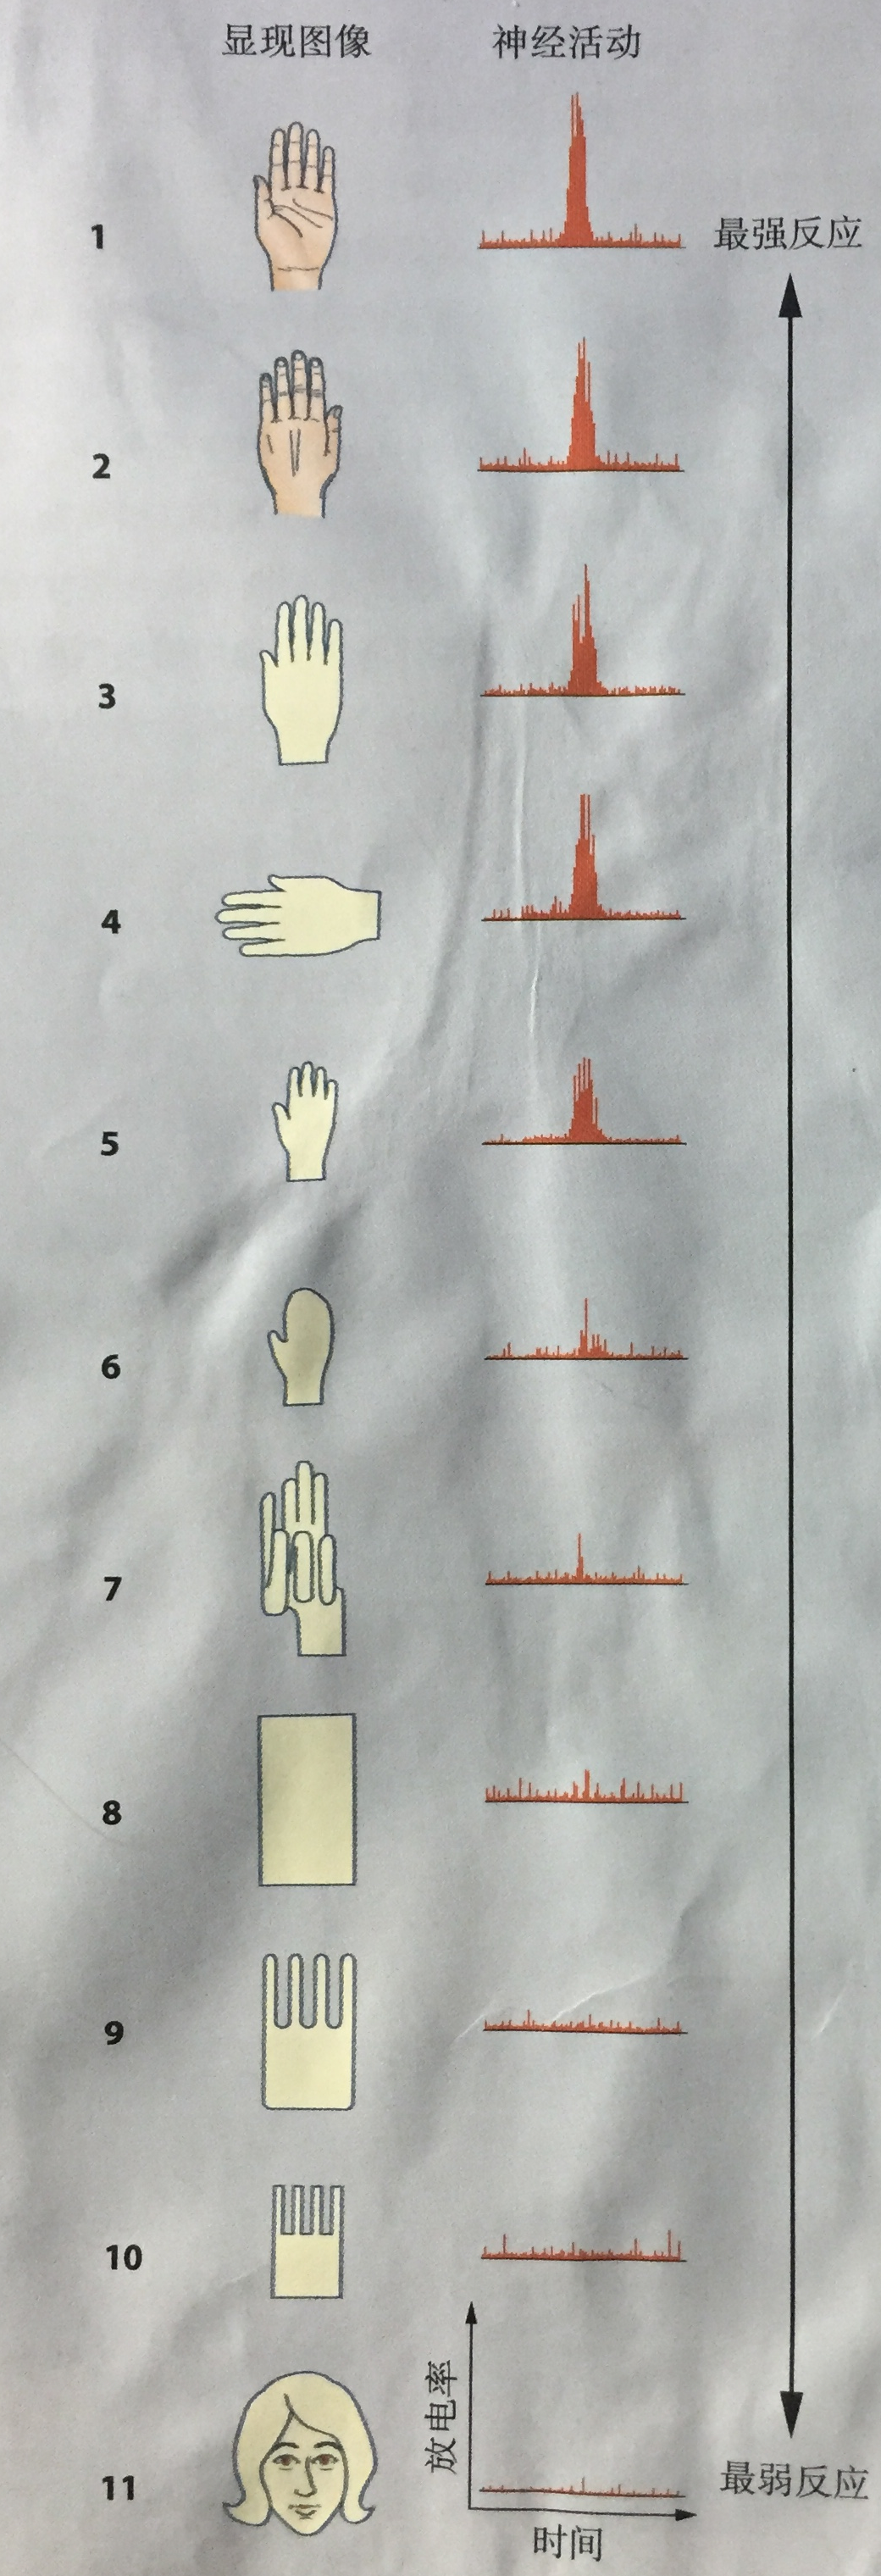
\includegraphics[width=0.1\textwidth]{/home/strawberryfg/brain/hand.png}
\caption{\cite{main}中对下颞皮质的一个神经元的单细胞记录}
\end{figure}\par 
	按照集群假说,检测手是多个神经元共同作用完成的。事实上,在检测手这个问题上,某些算法已经能达到非常好的效果,对于每一个像素都能将其分为属于手或者不属于手,在手的边界处也能较为精准地把手指和背景区别开,检测出的手和真实的手区域重合度非常高。\par 
	然而对于手的识别这个问题,算法远达不到大脑的效果。在大脑中,视觉系统的输入是三维的场景,投射到视网膜后的是二维成像,我们最后感知到的仍是三维的手。尽管可能存在自遮挡,某些手指可能会被另一些手指覆盖住,而且不同手指之间其实是非常相似的,此外手可能会在短时间内快速地全局旋转,但我们的大脑仍能区分不同的手指,精确地知道每一个手关节在三维场景中的具体位置,让我们感知到一个精准的手模型。从这个角度上说,大脑识别手的能力比算法强太多。那么,大脑是如何识别具体手势的呢?这又回到了物体识别的认知问题上,心理学家有不同的假说。一种假设是物体识别依赖于我们从某一个角度对物体的观察,在大脑的记忆里存储了一个物体从不同视角观察到的图像的视觉特征,在这个例子中,大脑保存了从不同角度观察手的图像表征,当新来一只手的时候我们只要去和记忆中的手表征匹配,匹配成功的就是识别出来的手。但是这种模型势必加重了大脑的记忆负荷,如果对所有的新物体都要存储各种视角的图像,我们一生会接触无数的物体,这种记忆负载是非常大的。另一种假设认为,物体识别加工有一个参照系,不依赖于观察角度,例如Marr(1982)假设知觉系统首先定义一个物体的主轴及次主轴,然后再参照这些轴定义物体的其它性质进行加工。根据这一假设,在手识别这个问题上可以理解为,视觉系统根据视网膜上关于手的二维成像提取出手的三维模型,并存储其不依赖于观察角度或物体实际尺寸的表征,达到所谓的\textbf{旋转不变性}和\textbf{尺度不变性}。一个手可以由20-50个自由度表示,也可以用若干球模型或者别的模型表示,从自由度到手模型之间存在唯一确定的对应变换关系,根据自由度,手模型可以绕着固定的x,y,z轴以及固定的三维空间中的点作旋转变换。如果知觉系统能针对手自动确定若干旋转轴,再定义其它自由度或者别的性质,即能完成手的加工与识别。当然,这只是一个假设。\par 
	笔者利用神经网络针对手势识别这一问题做过一些实验,神经网络处理手势的思路分成两种,一种是生成一种中间的表达方式如关节点的二维概率分布图,然后利用其它搜索方法从二维还原成三维,另外一种思路是直接输出是三维手各个关节在三维空间中的坐标,这样可以直接还原出三维的手模型,当然还有一些别的将观察到的手和我们对手模型的先验知识融合起来的混合神经网络。不管是哪种思路,它都不能处理大脑能轻松自如应对的自遮挡、自相似部位(手指相似)、手的全局快速移动等问题,与大脑相比相距甚远。然而,笔者输出了网络每层的神经元输出,发现一些有趣的现象。如下图,从左到右依次为网络第一、二、三层的输出结果。
\begin{figure}[htbp]
\centering
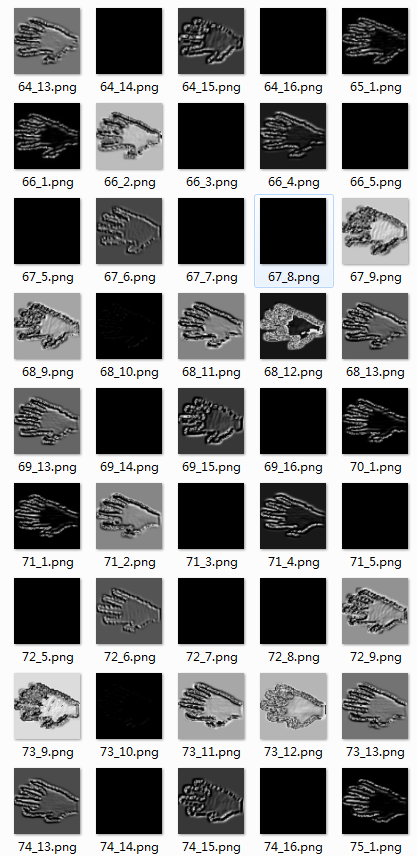
\includegraphics[width=0.307\textwidth]{/home/strawberryfg/brain/11.png}
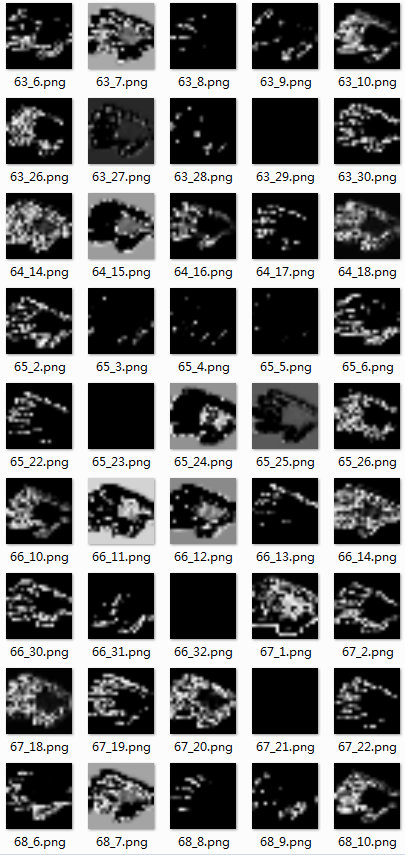
\includegraphics[width=0.30\textwidth]{/home/strawberryfg/brain/33.png}
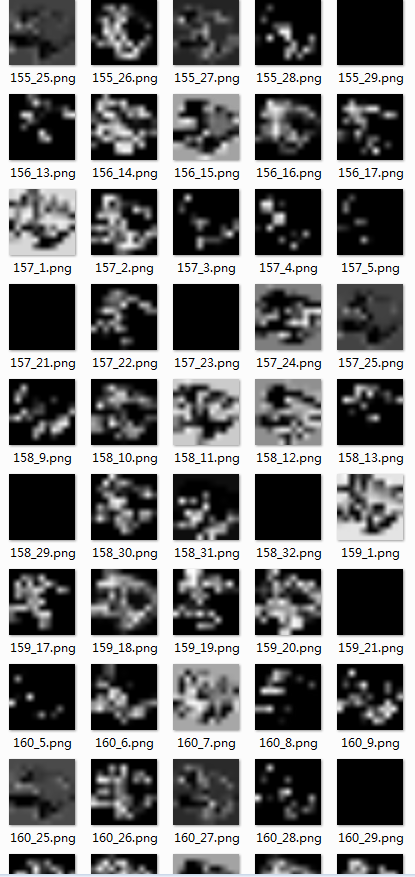
\includegraphics[width=0.295\textwidth]{/home/strawberryfg/brain/44.png}
\caption{1-5列为第一层输出,6-10列为第二层输出,11-15列为第三层输出}
\end{figure}\par 
	值得注意的是,第一层的结果可以说提取出了手的整个边界线,过滤了被边界包络住的手平面,第二层的结果较第一层而言显得更加杂乱无章,有些滤波器输出的图保留了大部分边缘,有些图几乎只有零散的手指尖部的几个点,有些在手指部位响应较为密集,而在其它部位没有响应。总而言之,第二层的输出不能简单的用边缘、拐角、形状等形容。可以发现在第二层还能隐约辨认出手的形状,但是第三层的输出则完全辨别不出手的特征,第三层的输出更像有若干个峰的二维高斯概率分布图,其中在每个峰附近集中了一些点。神经网络的更高层神经元整合了来自低层神经元的简单信息,经过精细加工表征更高阶的需要挖掘的信息,这些信息不是一眼就能辨识出来的。\par 
	关于神经网络每一层输出的信息有何含义,Matthew D. Zeiler和Rob Fergus在ECCV2014上的一篇论文\cite{visualize}中可视化输出了神经网的中间层如下图。(图中每个层对应了两幅图,第一幅为神经网的结果,第二幅为输入的原图)
 \begin{figure}[htbp]
\centering
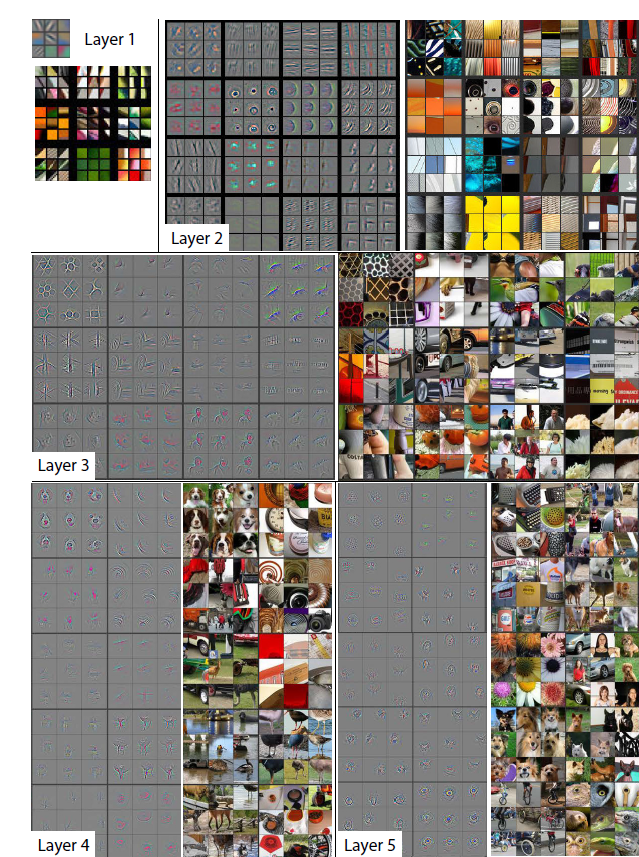
\includegraphics[width=0.8\textwidth]{/home/strawberryfg/brain/visualize.png}
\caption{\cite{visualize}可视化输出}
\end{figure}\par 	
	
	
	可以从图中看出:\par 
	1)Layer 2包含了拐角、边缘/颜色结合的信息\par 
	2)Layer 3有更复杂的不变性(invariance),不难发现,同一个物体比如同样的轮胎对应的输出图已经相对比较类似(类似物体的恒常性),这一层能获取相同的纹理(比如第一行第一列的网状条纹(mesh pattern),第二行第四列的文本(text))\par 
	3)Layer 3强调纹理不变性,而Layer 4强调变异性(variation),对物体的分类更具体了,神经网输出的图能看出图不同部位显著的差异。比如同是狗,第一行第一列的9个狗脸各不相同,第四行第二列的鸟腿也是如此。\par 
	4)Layer 5的物体有更加显著的不同(比如第一行第一列的各个键盘,第四行的各种狗) 。\par 
	综上所述,既然初级视皮质简单细胞负责边界,高级细胞表征拐角和边缘终端等更复杂信息,在更高层的视皮质区负责形状以及更高级的特征,神经网络的神经元的响应也很类似生物的这种机制,低层有边缘信息,然后中间的层有拐角、纹理信息,更高层有更抽象复杂的高阶特征,那么能否认为神经网络已经能很好地模拟大脑神经元的运作了呢?倘若就此下定论恐怕还为时过早,毕竟神经网络是工程、数学上的内容,归根到底还是在做一个数值优化问题,与大脑里复杂的树突轴突网、神经回路相比,即使Google的识别物体的19层网络GoogleNet以及MSRA的152层网络\cite{deep}也是小巫见大巫,Google的DeepMind项目组一直在试图用更深的网络模拟大脑的数以亿计的神经元,然而我们真的需要使计算机完全达到人脑的水平吗?可以预见在一个很长的时间内,神经网络基本完全模拟大脑都是不太可能发生的。笔者认为,我们不是要尽可能的模仿大脑,相似度越高越好,大脑作为一个非常精细的部件,人类对其的认知还非常有限,我们没有必要也不可能完全模拟生产另一个大脑。生物神经科学有它的研究思路,神经网络则是另一套思路,在还没有完全了解清楚大脑内部神经系统的构造情况下,直接借鉴恐怕不是一个好的选择。
\section{总结}
\ \ \ \ 人类对物体的认知能力是无穷的,要识别物体,我们的视觉系统需要有极高的处理加工和组合能力。经过漫长的进化,人类的视觉系统已经达到非常成熟的阶段。通过本文对视网膜、外侧膝状体和皮质视觉区这一整条视觉神经传导通路的综述,我们可以看到视觉信息经过不同的区域同时并行地专门化处理,能够提取出低阶的边界和高阶的轮廓、形状、纹理等抽象的特征,这些特征表征了不同的物体,能够克服输入的内在变异性。不同的皮质视觉区相互协作,共同组成了视觉感知系统。\par 
	此外,除了皮质视觉区,大脑特定区域在物体识别中也起到了关键作用。从神经水平的整体角度考虑,物体在大脑中有两种表征方式,一种假说认为物体识别是由单个神经元完成的,而另一种假说认为物体识别是由多个神经元共同作用完成的,后者得到了实验的验证。部分学者认为只考虑知觉特征对识别物体而言是不够的,还需将视觉系统加工的知觉特征和我们记忆中储存的关于物体的语义知识结合起来,据此提出了一些知觉和语义融合的认知模型。针对物体特征的加工阶段,有人提出了整体加工和分析加工的双加工模型。\par 
	物体识别这个问题在计算机视觉领域取得了广泛的关注,许多科研人员试图通过神经网络模拟大脑神经元,本文结合笔者自身的实验感悟简单分析了神经网络处理这个问题的缺陷和不足,指出神经网络目前来说仅仅是简单地借用了神经元的概念,并不能很好地模拟大脑神经系统,同时说明了大脑识别物体的精妙之处。\par 	
	人类的大脑具有极强的分析和组合能力,能把经过视觉神经传导通路加工处理过的亮度、形状、颜色、纹理、运动方向、运动速度、深度等各种抽象的知觉信息在更高的层次上进行概括和整合,最终形成完整的视知觉,帮助人类感知世界。随着神经生物学的发展,视觉神经传导通路、视觉信息处理和物体识别的研究还将进一步深入。本综述还存在很多不足的地方值得进一步改进。
\renewcommand\refname{参考文献}
\bibliographystyle{plain}
\bibliography{brain}
\end{document}
\end{CJK}{UTF8}{gkai}